% 最小二乘法的数值计算
% 最小二乘法|数值拟合|极小值

\pentry{最小二乘法\upref{LstSqr}, Nelder-Mead 算法\upref{NelMea}}
我们在 “最小二乘法\upref{LstSqr}” 见到的三个例子中, 方差函数都是待定系数的线性组合, 这种情况下我们令偏导为零后得到的是线性方程组, 便于求解%(见 Matlab 或 Mathematica)链接未完成. 
. 然而当方差不是待定系数的线性组合时, 得到的方程组往往非常复杂, 这时就需要借助数值计算. 相比用数值计算解 $N$ 元的非线性方程组, 更简单的方法是直接用数值方法寻找方差函数的极小值(如Nelder-Mead 算法) . 实践证明, 大多数情况下极小值点仅有一个, 那就是最小值点.

为了验证结果的正确性, 我们先来用数值方法拟合 $A\cos (x + \varphi_0) + C$, 并与“最小二乘法\upref{LstSqr}” 中的方法比较结果.

\begin{figure}[ht]
\centering
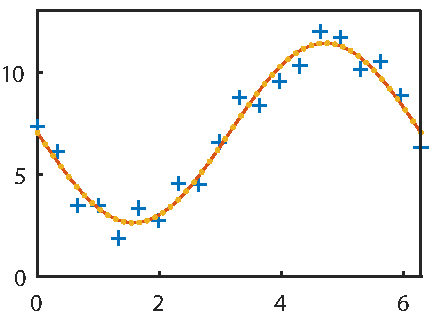
\includegraphics[width=8cm]{./figures/CurFit_1.pdf}
\caption{运行结果} \label{CurFit_fig1}
\end{figure}

\subsubsection{curveFit.m}
\begin{lstlisting}[language=matlab]
function curveFit
close all;
% 随机生成简谐曲线
N = 20;
x0 = linspace(0, 2*pi, N);
y0 = 5*rand * sin(x0 + 2*pi * rand) + 10 * rand;
y0 = y0 + 2*rand(1,20); % 产生随机误差
scatter(x0, y0, '+'); % 画出散点
hold on;

% Nelder-Mead 求方差最小值点
f = @(x) norm( x(1)*sin(x0 + x(2)) + x(3) - y0 )^2;
c = NelderMead(f, [5, 1, 5], 1e-7);
% 画拟合结果
x = linspace(0, 2*pi, 50);
y1 = c(1) * sin(x + c(2)) + c(3);
plot(x, y1);

% 解线性方程组求方差最小值点
c = sinfit(x0, y0);
% 画拟合结果
y2 = c(1)*cos(x) + c(2)*sin(x) + c(3);
plot(x, y2, '.');
end

% 拟合简谐曲线
% y = C(1)*cos(x) + C(2)*sin(x) + C(3)
function C = sinfit(x, y)
N = numel(x);
cosx = cos(x); sinx = sin(x);
sc = sum(sinx.*cosx);
s = sum(sinx); c = sum(cosx);
% 系数矩阵
M = [sum(cosx.^2), sc          , c;
               sc, sum(sinx.^2), s;
                c,            s, N];
b = [sum(y.*cosx); sum(y.*sinx); sum(y)];
C = M\b; % 解线性方程组
end
\end{lstlisting}

运行结果如\autoref{CurFit_fig1} 所示, 可见两种方法拟合出的曲线一致(红色的曲线和黄色的点线). 注意第 13 行使用了“Nelder-Mead 算法\upref{NelMea}” 中的函数 \lstinline|NelderMead| 求函数句柄 \lstinline|f| 的最小值.
